\documentclass[conference]{IEEEtran}
\IEEEoverridecommandlockouts
% The preceding line is only needed to identify funding in the first footnote. If that is unneeded, please comment it out.
\usepackage{cite}
\usepackage{amsmath,amssymb,amsfonts}
\usepackage{algorithmic}
\usepackage{graphicx}
\usepackage{textcomp}
\usepackage{xcolor}

\usepackage{xspace}
\setlength{\marginparwidth}{2cm}
\usepackage{todonotes}
\usepackage[normalem]{ulem}
\usepackage{glossaries}
\usepackage{paralist}
\usepackage{url}
\usepackage{natbib}

%% Abbreviations and short helpers
\def\figref#1{Fig.~\ref{#1}}
\newcommand{\babsimhospital}{\textsc{BaBSim.Hospital}\xspace} 
%\newcommand{\spot}{\textsc{SPOT}\xspace}
%\newcommand{\spo}{\textsc{SPO}\xspace}
\newcommand{\simmer}{\textsc{simmer}\xspace}


%% Acronyms
\newacronym{CI}{CI}{Continuous Integration}
\newacronym{CICD}{CI/CD}{Continuous Integration / Continuous Deployment}
\newacronym{CD}{CD}{Continuous Deployment}
\newacronym{COVID-19}{COVID-19}{Coronavirus disease 2019}
\newacronym{DES}{DES}{Discrete Event Simulation}
\newacronym{DIVI}{DIVI}{Deutsche interdisziplinäre Vereinigung für Intensiv- und Notfallmedizin}
\newacronym{ECiP}{ECiP}{Evolutionary Computation in Practice}
\newacronym{EGO}{EGO}{Efficient Global Optimization}
\newacronym{ETL}{ETL}{Extract, Transform, and Load}
\newacronym{ICU}{ICU}{Intensive Care Unit}
\newacronym{LHD}{LHD}{Latin Hypercube Design}
\newacronym{R}{R}{R language and environment for statistical computing and graphics}
\newacronym{RKI}{RKI}{Robert Koch Institute}
\newacronym{RMSE}{RMSE}{Root Mean Squared Error}
\newacronym{RSM}{RSM}{Response surface methodology}
\newacronym{simmer}{simmer}{``Discrete-Event Simulation for R''}
\newacronym{SHERPA}{SHERPA}{Simultaneous Hybrid Exploration that is Robust, Progressive and Adaptive}
\newacronym{SMBO}{SMBO}{Surrogate Model-Based Optimization}
\newacronym{SMBSA}{SMBSA}{Surrogate Model-Based Sensitivity Analysis}
\newacronym{SPOT}{SPOT}{Sequential Parameter Optimization Toolbox}







\def\BibTeX{{\rm B\kern-.05em{\sc i\kern-.025em b}\kern-.08em
    T\kern-.1667em\lower.7ex\hbox{E}\kern-.125emX}}

\renewenvironment{description}[0]{\begin{compactdesc}}{\end{compactdesc}}

\begin{document}

\title{Optimization and Adaptation of a Resource Planning Tool for Hospitals Under Special Consideration of the COVID-19 Pandemic
\thanks{Identify applicable funding agency here. If none, delete this.}
}

\author{
\IEEEauthorblockN{
Thomas Bartz-Beielstein\IEEEauthorrefmark{1},
Marcel Dröscher\IEEEauthorrefmark{2},
Alpar Gür\IEEEauthorrefmark{3},
Alexander Hinterleitner\IEEEauthorrefmark{4},}
\IEEEauthorblockN{
Olaf Mersmann\IEEEauthorrefmark{5}, % bin dabei!
Dessislava Peeva\IEEEauthorrefmark{6},
Lennard Reese\IEEEauthorrefmark{7},
Nicolas Rehbach\IEEEauthorrefmark{8},
}
\IEEEauthorblockN{
Frederik Rehbach\IEEEauthorrefmark{9},
Amrita Sen\IEEEauthorrefmark{10},
Aleksandr Subbotin\IEEEauthorrefmark{11} and
Martin Zaefferer\IEEEauthorrefmark{12}
}
\IEEEauthorblockA{
\textit{Inst. Data Science, Engineering, and Analytics} \\
\textit{TH Köln}, Cologne, Germany \\
ORC-ID / Email:
\IEEEauthorrefmark{1}\url{https://orcid.org/0000-0002-5938-5158},
\IEEEauthorrefmark{2}marcel\_ulrich.droescher@smail.th-koeln.de,\\
\IEEEauthorrefmark{3}alpar.guer@smail.th-koeln.de,
\IEEEauthorrefmark{4}Alexander.Hinterleitner@th-koeln.de,
\IEEEauthorrefmark{5}olaf.mersmann@th-koeln.de,\\
\IEEEauthorrefmark{6}dessislava\_todorova.peeva@smail.th-koeln.de,
\IEEEauthorrefmark{7}lennard.reese@smail.th-koeln.de,\\
\IEEEauthorrefmark{8}nicolas\_alexander.rehbach@smail.th-koeln.de,
\IEEEauthorrefmark{9}frederik.rehbach@th-koeln.de,
\IEEEauthorrefmark{10}amrita.sen@gmx.de,\\
\IEEEauthorrefmark{11}aleksandr.subbotin@smail.th-koeln.de,
\IEEEauthorrefmark{12}martin.zaefferer@th-koeln.de
}
}

\maketitle

\begin{abstract}
Crises like the COVID-19 pandemic pose a serious challenge to health-care institutions. They need to plan the resources required for handling the increased load, for instance, hospital beds and ventilators. To support the resource planning of local health authorities from the Cologne region, \babsimhospital, a tool for capacity planning based on discrete event simulation,  was created. The predictive quality of the simulation is determined by 29 parameters. Reasonable default values of these parameters were obtained in detailed discussions with medical professionals.  We aim to investigate and optimize these parameters to improve \babsimhospital. First approaches with "out-of-the-box" optimization algorithms failed. Implementing a surrogate-based optimization approach generated useful results in a reasonable time. 
The adaptation has been shown to reduce simulation errors by nearly 70\%

The presented approach is applicable to many other real-world problems, e.g., the development of new elevator systems to cover the last mile or simulation of student flow in academic study periods.
\end{abstract}

\begin{IEEEkeywords}
optimization-via-simulation, surrogate-model-based optimization, sensitivity analysis, COVID-19, hospital resource planning, prediction tool, capacity planning
\end{IEEEkeywords}


\section{Introduction}\label{sec:intro}
Our initiative is motivated by the challenges that health care institutions face in the current COVID-19 pandemic. 
Planning the demand and availability for specific resources, such as intensive care beds, ventilators, and staff resources, is crucial.
Policies and decisions made by hospital management professionals as well as political officials need to be well informed to be effective.

This article reports the experiences that were collected over the last 12 months and provides answers to the following questions:
\begin{compactenum}[(Q-1)]
\item How to select a suitable simulation model?
\item How to find an optimization algorithm that is able to solve noisy, dynamic, high-dimensional real-world problems?
\item How to extend the interface  that enables  usage  of  data  independently  from  the German DIVI  and  RK?
\item How to integrate domain knowledge and how to adapt a complex simulation model to a new environment?
\end{compactenum}
In the following, a holistic approach that demonstrates how tools from evolutionary optimization, simulation, sensitivity analysis, and machine learning can be combined to predict and understand demanding resource allocation problems is presented.
We illustrate how the pieces can be put together in a complex software project, i.e., we consider the collection of noisy, dynamic, and heterogeneous data, data preprocessing, surrogate models to accelerate simulation, the optimization of the model parameters, and a parameter sensitivity analysis.

Simulation models are valuable tools for resource usage estimation and capacity planning.
They can either be implemented top down, e.g., using time series approaches~\cite{Hynd08b} or bottom up, e.g., using \gls{DES}~\cite{Bank01a}.
Benefits of \gls{DES} are manifold and range from providing insights into the process’s risk and efficiency when estimating the effects of alternating configurations of the system.
It helps to gain insight into consequences of redesign strategies.
\gls{DES} has been successfully applied to problems that model customers arriving at a bank,   
products being manipulated in a supply chain, and the performance of configurations of a telecommunications network~\cite{Bank01a}.

This bottom-up approach, i.e., a \gls{DES}, is used to model the hospital resource planning problem.
\babsimhospital simulates the path of many thousands or possibly even millions of patient trajectories through hospitals.
This simulation requires considerable computational resources.
Therefore, a very efficient simulator is required, since only a limited number of simulations can be performed in a reasonable time frame.
We have chosen \gls{simmer}, a \gls{DES} package which enables high-level process-oriented modeling~\citep{Ucar19a}. 
The code required for running the simulations is published as an open-source R-Package~\citep{bart20rArxiv, bart20t}.

\gls{simmer} is based on the concept of a trajectory: a common path in the simulation model for entities of the same type.
Trajectories consist of a list of standardized actions, which define the life cycle of equivalent processes. 
It takes available hospital data into account and offers hospitals and policymakers a means to simulate the progression of the pandemic in terms of available and occupied hospital resources and capacity. 
The modeling approach is inspired by~\citet{Lawt19a} and is enhanced by a  \gls{SMBO} approach~\citep{Forr08a}, i.e., our system 
combines several powerful approaches: 
\begin{description}
    \item[Discrete event simulation:] the 'simmer' R-package is used to generate a simulation with 29 parameters with default values, established in cooperation with medical professionals~\citep{Ucar19a}. These parameters are essential for the accuracy of the simulation and require careful optimization. Although domain knowledge, i.e., from medical professionals, provides valuable information to perform realistic simulations, further fine-tuning is required.
    \item [Model-based optimization:] the  \gls{SPOT} R-package is used to perform  \gls{SMBO} to identify the best values for the 29 parameters in a fast and accurate manner, which results in an optimization-via-simulation approach~\cite{Fu94a}.
\end{description}
However, the relatively large number of parameters limits the quality of the optimization process. 

The rest of this paper is structured as follows: 
Section~\ref{sec:data} discusses the available data and its preparation,
Section~\ref{sec:sim} introduces the \babsimhospital simulator and 
Section~\ref{sec:optim} describes the corresponding optimization problem. 
Section~\ref{sec:adaptation} describes how domain knowledge can be used to adapt the search boundaries.
Specifically, we will discuss the availability of ventilated \gls{ICU} bed in Germany and in the UK: Compared to Germany, there is only a small number of ICU beds with ventilation in the UK.
Finally, the results of this project are discussed in Section~\ref{sec:discussion}.

\section{Automated Data Collection and Curation}\label{sec:data}
\babsimhospital combines data from two different sources:
\begin{compactenum}
\item simData: simulation data, i.e., input data for the simulation. The onlinve version of the \babsimhospital simulator use s data from the \gls{RKI}.
\item fieldData: real data, i.e., data from the DIVI-Intensivregister. The 
  field data will be used for validating the simulation output. 
\end{compactenum}
Statistically speaking, the \babsimhospital simulator models 
 resources usage in hospitals, e.g., number of \gls{ICU} beds ($y$), as a function 
of the number of infected individuals ($x$).
In addition to the number of infections, information about age and gender can be used as simulation input.

\gls{ETL} processes integrate data from various sources into complex collections. 
A typical problem is ``that each data source has its distinct set of characteristics 
that need to be managed in order to effectively extract data for the \gls{ETL} process''~\citep{ELSAPPAGH201191}. 
After the successful extraction of data, the next step is to transform it. 
This step includes several approaches to gain accurate data which is correct, complete, consistent, and unambiguous.  
The final step consists of loading the processed data into a data collection of choice accessible for the data analyst for further use.
Especially in terms of the COVID-19 pandemic, it is important to integrate and process the vast amount of constantly growing data. 

\subsubsection{Germany}


\begin{figure*}
    \centering
    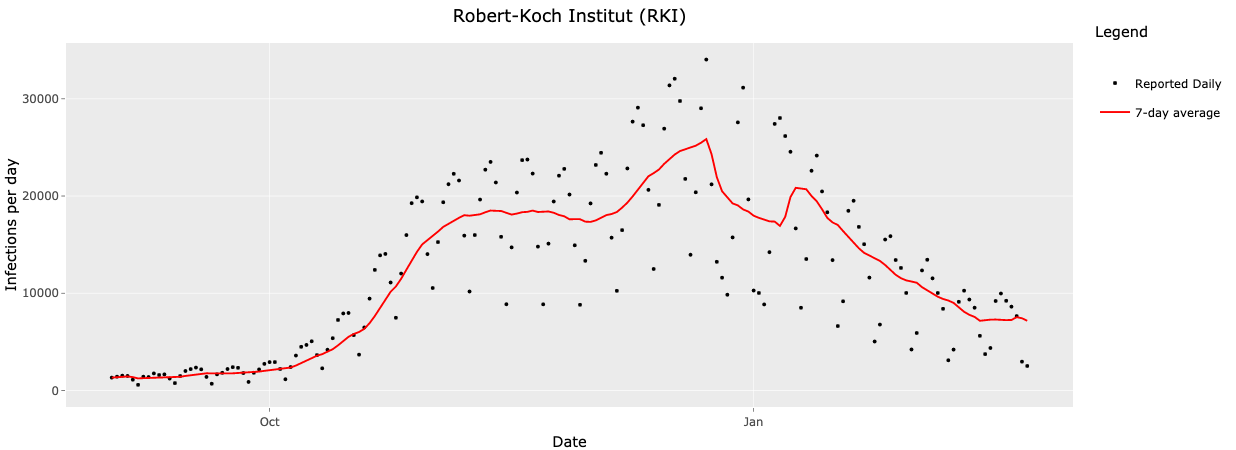
\includegraphics[width=0.75\linewidth]{infections.png}
    \caption{}
\label{fig:rki}
\end{figure*}

\begin{figure*}
    \centering
    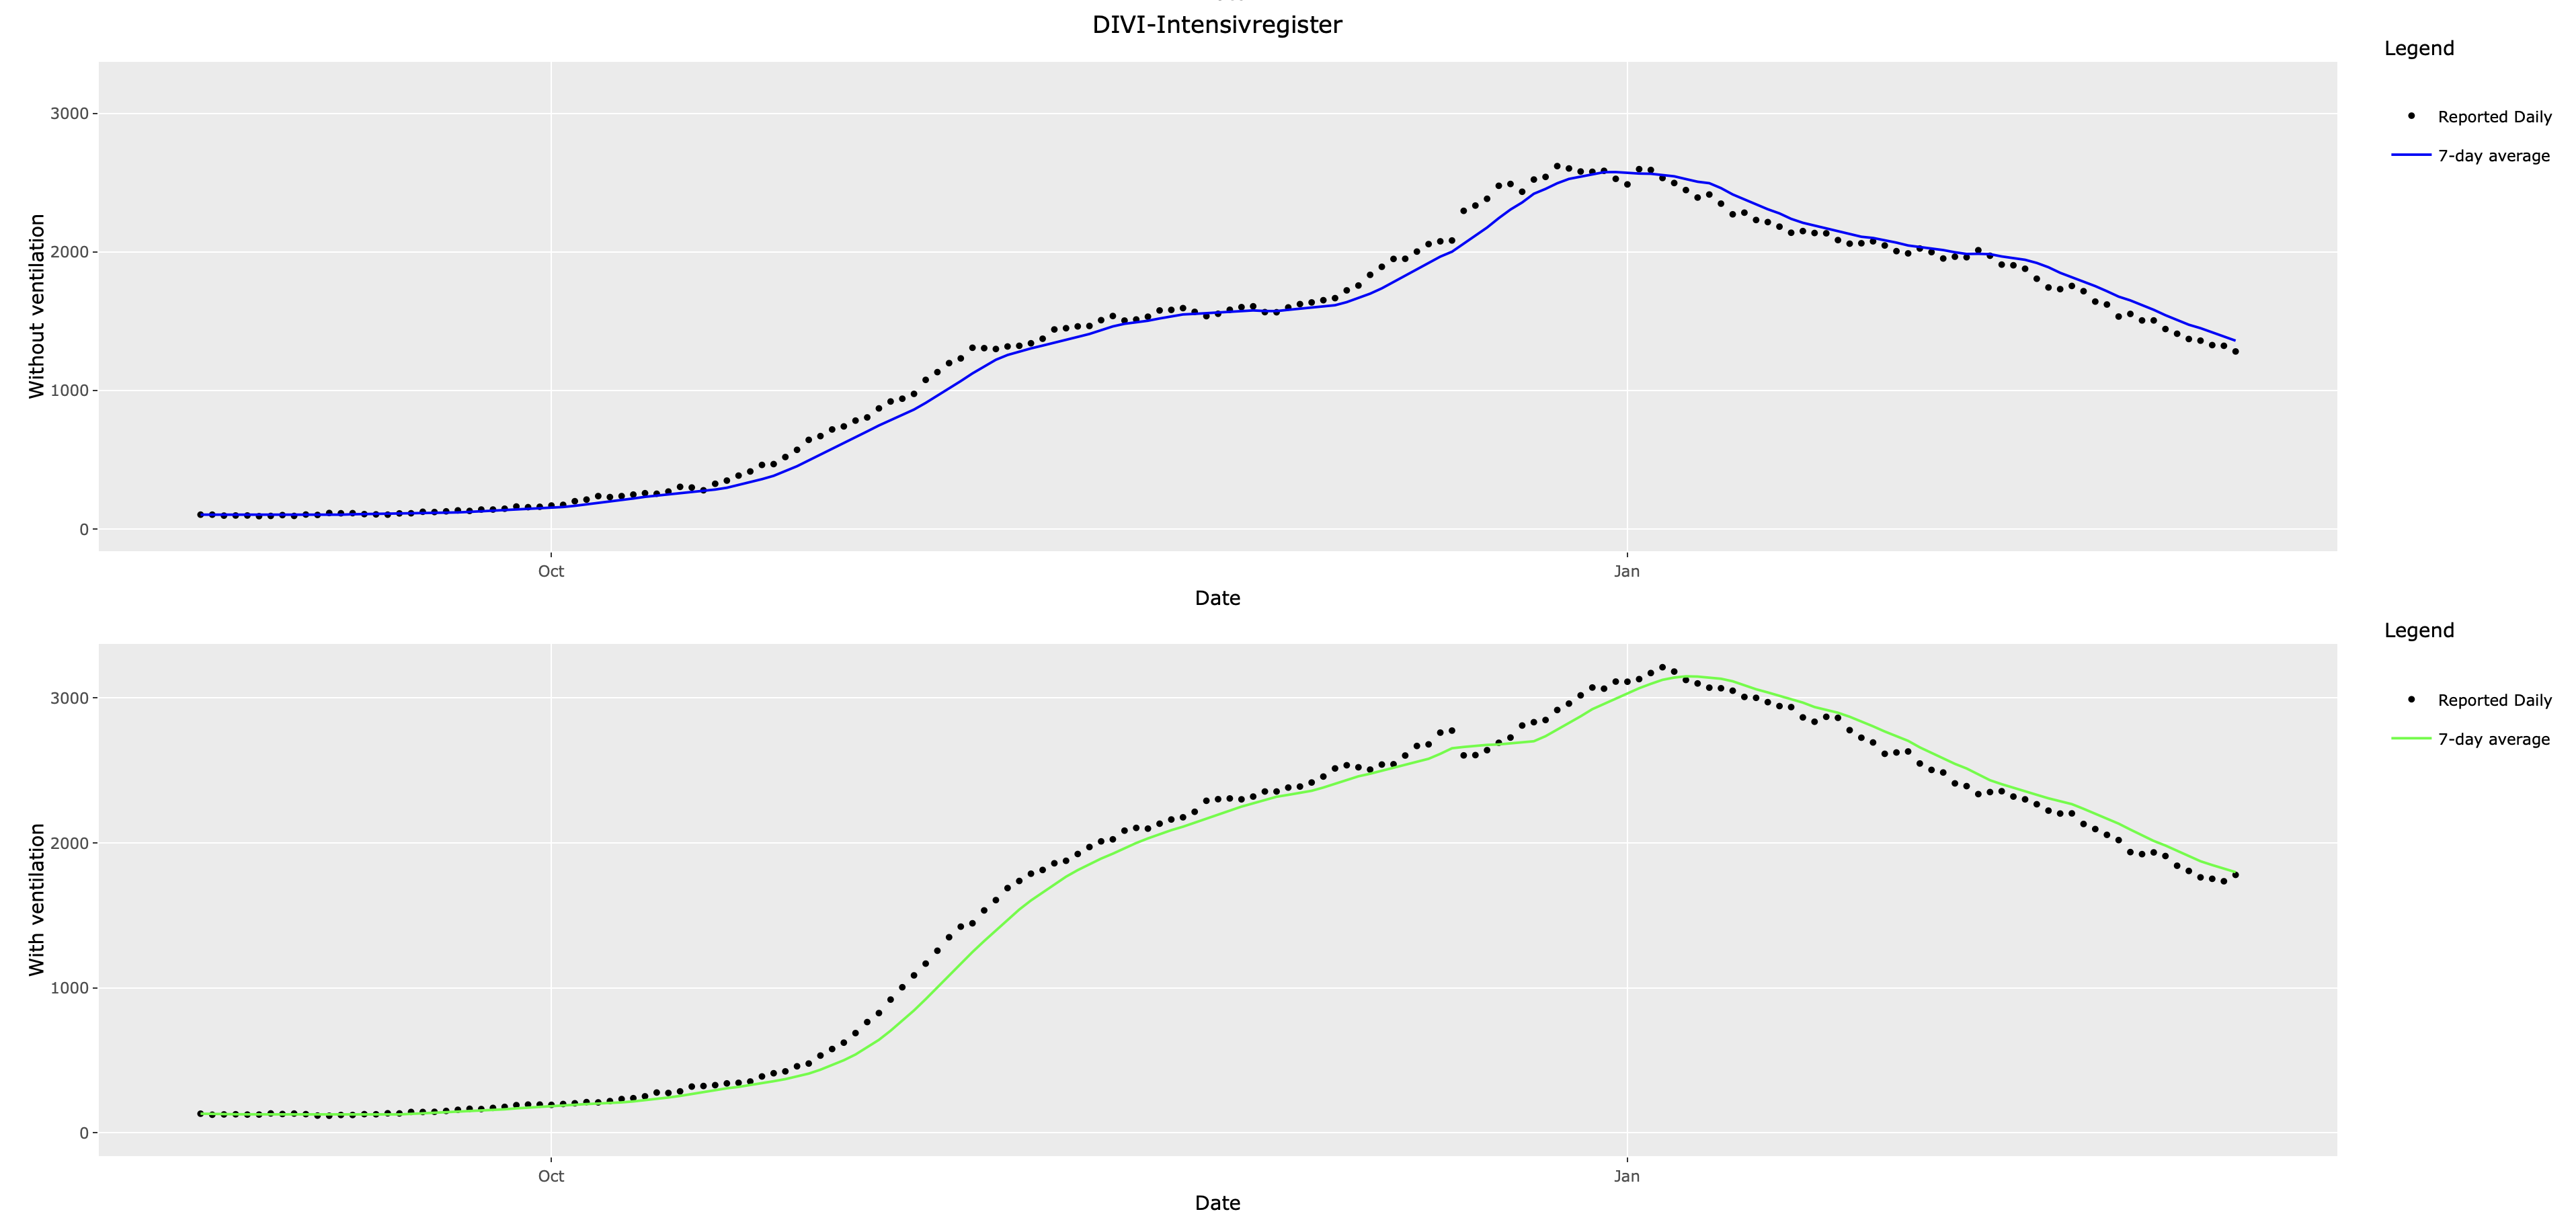
\includegraphics[width=0.75\linewidth]{dividata.png}
    \caption{}
\label{fig:divi}
\end{figure*}


\babsimhospital implements an \gls{ETL} process to analyze the data from the \gls{RKI}, \url{https://www.rki.de}, as well as the \gls{DIVI}, \url{https://www.divi.de}).
The associated data sets contain anonymous information about every recorded case in Germany. The \gls{RKI} data set contains 
780,065 observations of 18 variables such as age, gender, data of infection, etc., which were updated daily and are automatically integrated into \babsimhospital. 

Information concerning \gls{ICU} in Germany can be retrieved from the \gls{DIVI}.
\gls{DIVI} provides an API and a daily report. The API does not provide all data the daily report consists of and therefore is not a viable option for this project.
Web scraping was implemented as a reliable solution to retrieve the most current daily report from \gls{DIVI}.

The official simulator, which can be accessed via \url{https://www.th-koeln.de/babsimhospital}, uses \gls{DIVI} and \gls{RKI} data.
Its parameters are based on discussions with experts from Germany, especially \gls{ICU} doctors and experts from health administration.
The online version is described in Section~\ref{sec:online}.



\subsubsection{UK}
This paper describes an extension of the interface that enables usage of data independently from \gls{DIVI} and \gls{RKI} data, i.e., an interface to csv files and excel files can be uses so that any kind of field and simulation data can be processed, simulated, and optimized.
To demonstrated our approach, anonymised data from a region in the UK was used. 

Read data from Excel file.
The UK data consists of the following entries:
\begin{compactitem}
\item Date
\item bed: Total COVID inpatient = total in hospital (includes ICU)
\item intensiveBed: COVID-19 Non-invasive = patients on non-invasive ventilators (CPAP). In theory these should be on ICU but we don’t have space for them all. The model should probably consider them to be ICU but not intubated (level 2)
\item intensiveBedVentilation: COVID-19 Ventilated = patients ventilated and intubated on ICU
\end{compactitem}
The field data based on UK data used three bed categories: 
\begin{compactenum}
\item bed: non ICU patients in hospital
\item intensiveBed: ICU bed without ventilation
\item intensiveBedVentilation: \gls{ICU} bed with ventilation
\end{compactenum}
Figure~\ref{fig:ukdata} visualizes the UK data set that is used in this study. The whole data set consists of data from 240 days. Since our analysis considers the second \gls{COVID-19} wave only, we use data after after September 2020.
\begin{figure*}
    \centering
    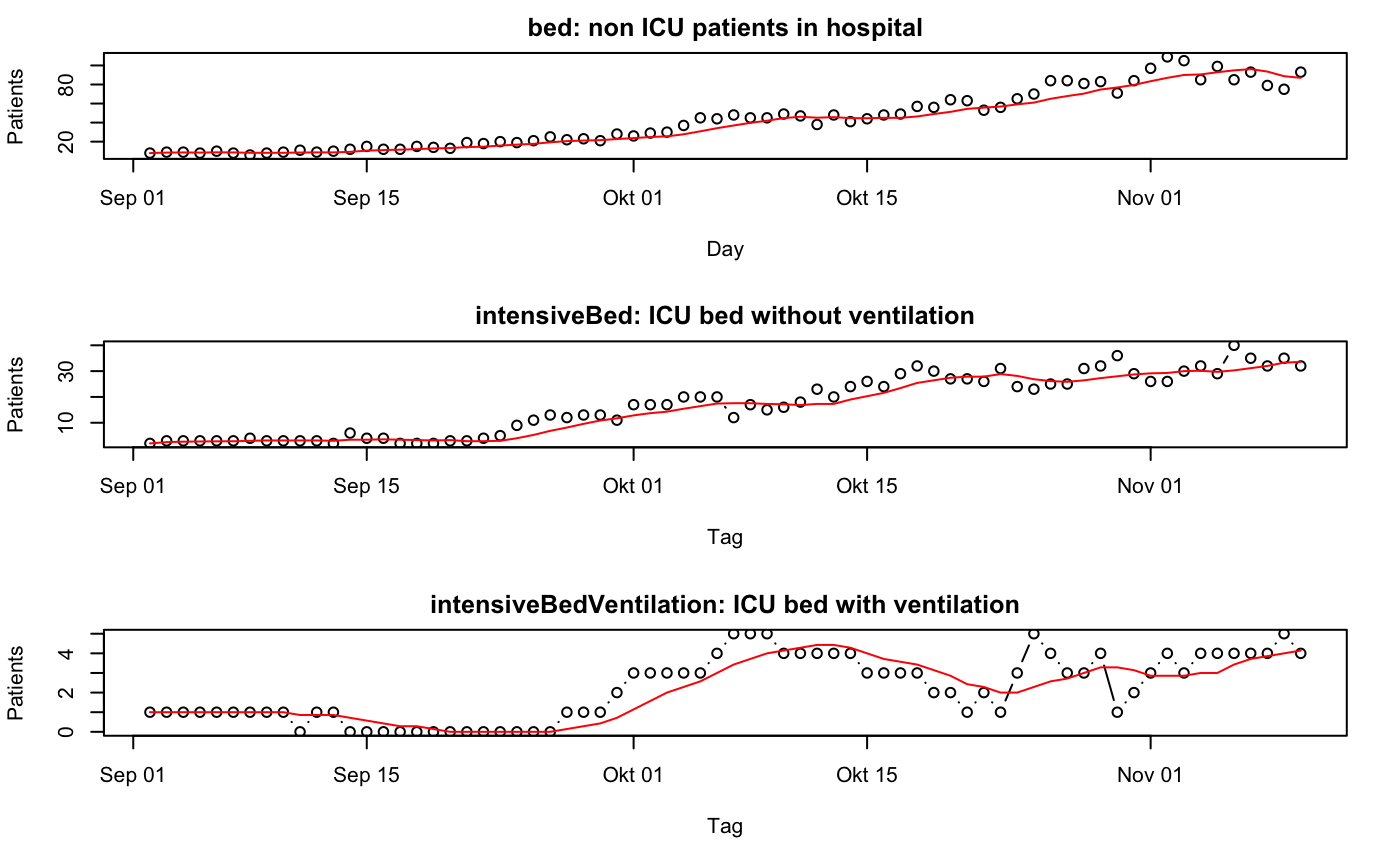
\includegraphics[width=0.75\linewidth]{ukdata3.png}
    \caption{UK data. Dots denote real-world data, red lines represent the seven-day average. \gls{ICU} beds with ventilation are shown in the last row. Compared to Germany, there is only a small number of \gls{ICU} beds with ventilation in the UK.}
\label{fig:ukdata}
\end{figure*}



\section{The Simulator}\label{sec:sim}
\subsection{Discrete Event Simulation}
\babsimhospital simulates the typical paths that COVID-19 infected patients follow during their hospital stays. 
The \gls{DES} processes every single recorded infection until the patients' recovery or death. 
Patients follow a trajectory, i.e., they move with a probability $p_{ij}$ from state $S_i$ to state $S_j$  after a transition-specific duration $d_{ij}$.
\babsimhospital includes tools to analyse parameter settings.
Parameter settings consist of
\begin{compactitem}
\item transition probabilities, e.g., the probability that an infected
   individual has to go to the hospital. 
\item  durations, e.g., the time span until an infected individual goes to the
   hospital (in days). 
\end{compactitem}
A graph can be used to model this behavior.
Figure~\figref{fig:prob} illustrates the transition probabilities.
The states are as follows:
\begin{compactenum}
\item infec: infected
\item out: transfer out, no hospital required
\item hosp: hospital
\item normal: normal station, no ICU
\item intens: ICU (without ventilation)
\item vent: ICU ventilated
\item intafter: intensive aftercare (from ICU with ventilation, on ICU)
\item aftercare: aftercare (from ICU,  on normal station)
\item death: patient dies
\item healthy: recovered
\end{compactenum}
 



\begin{figure*}
    \centering
    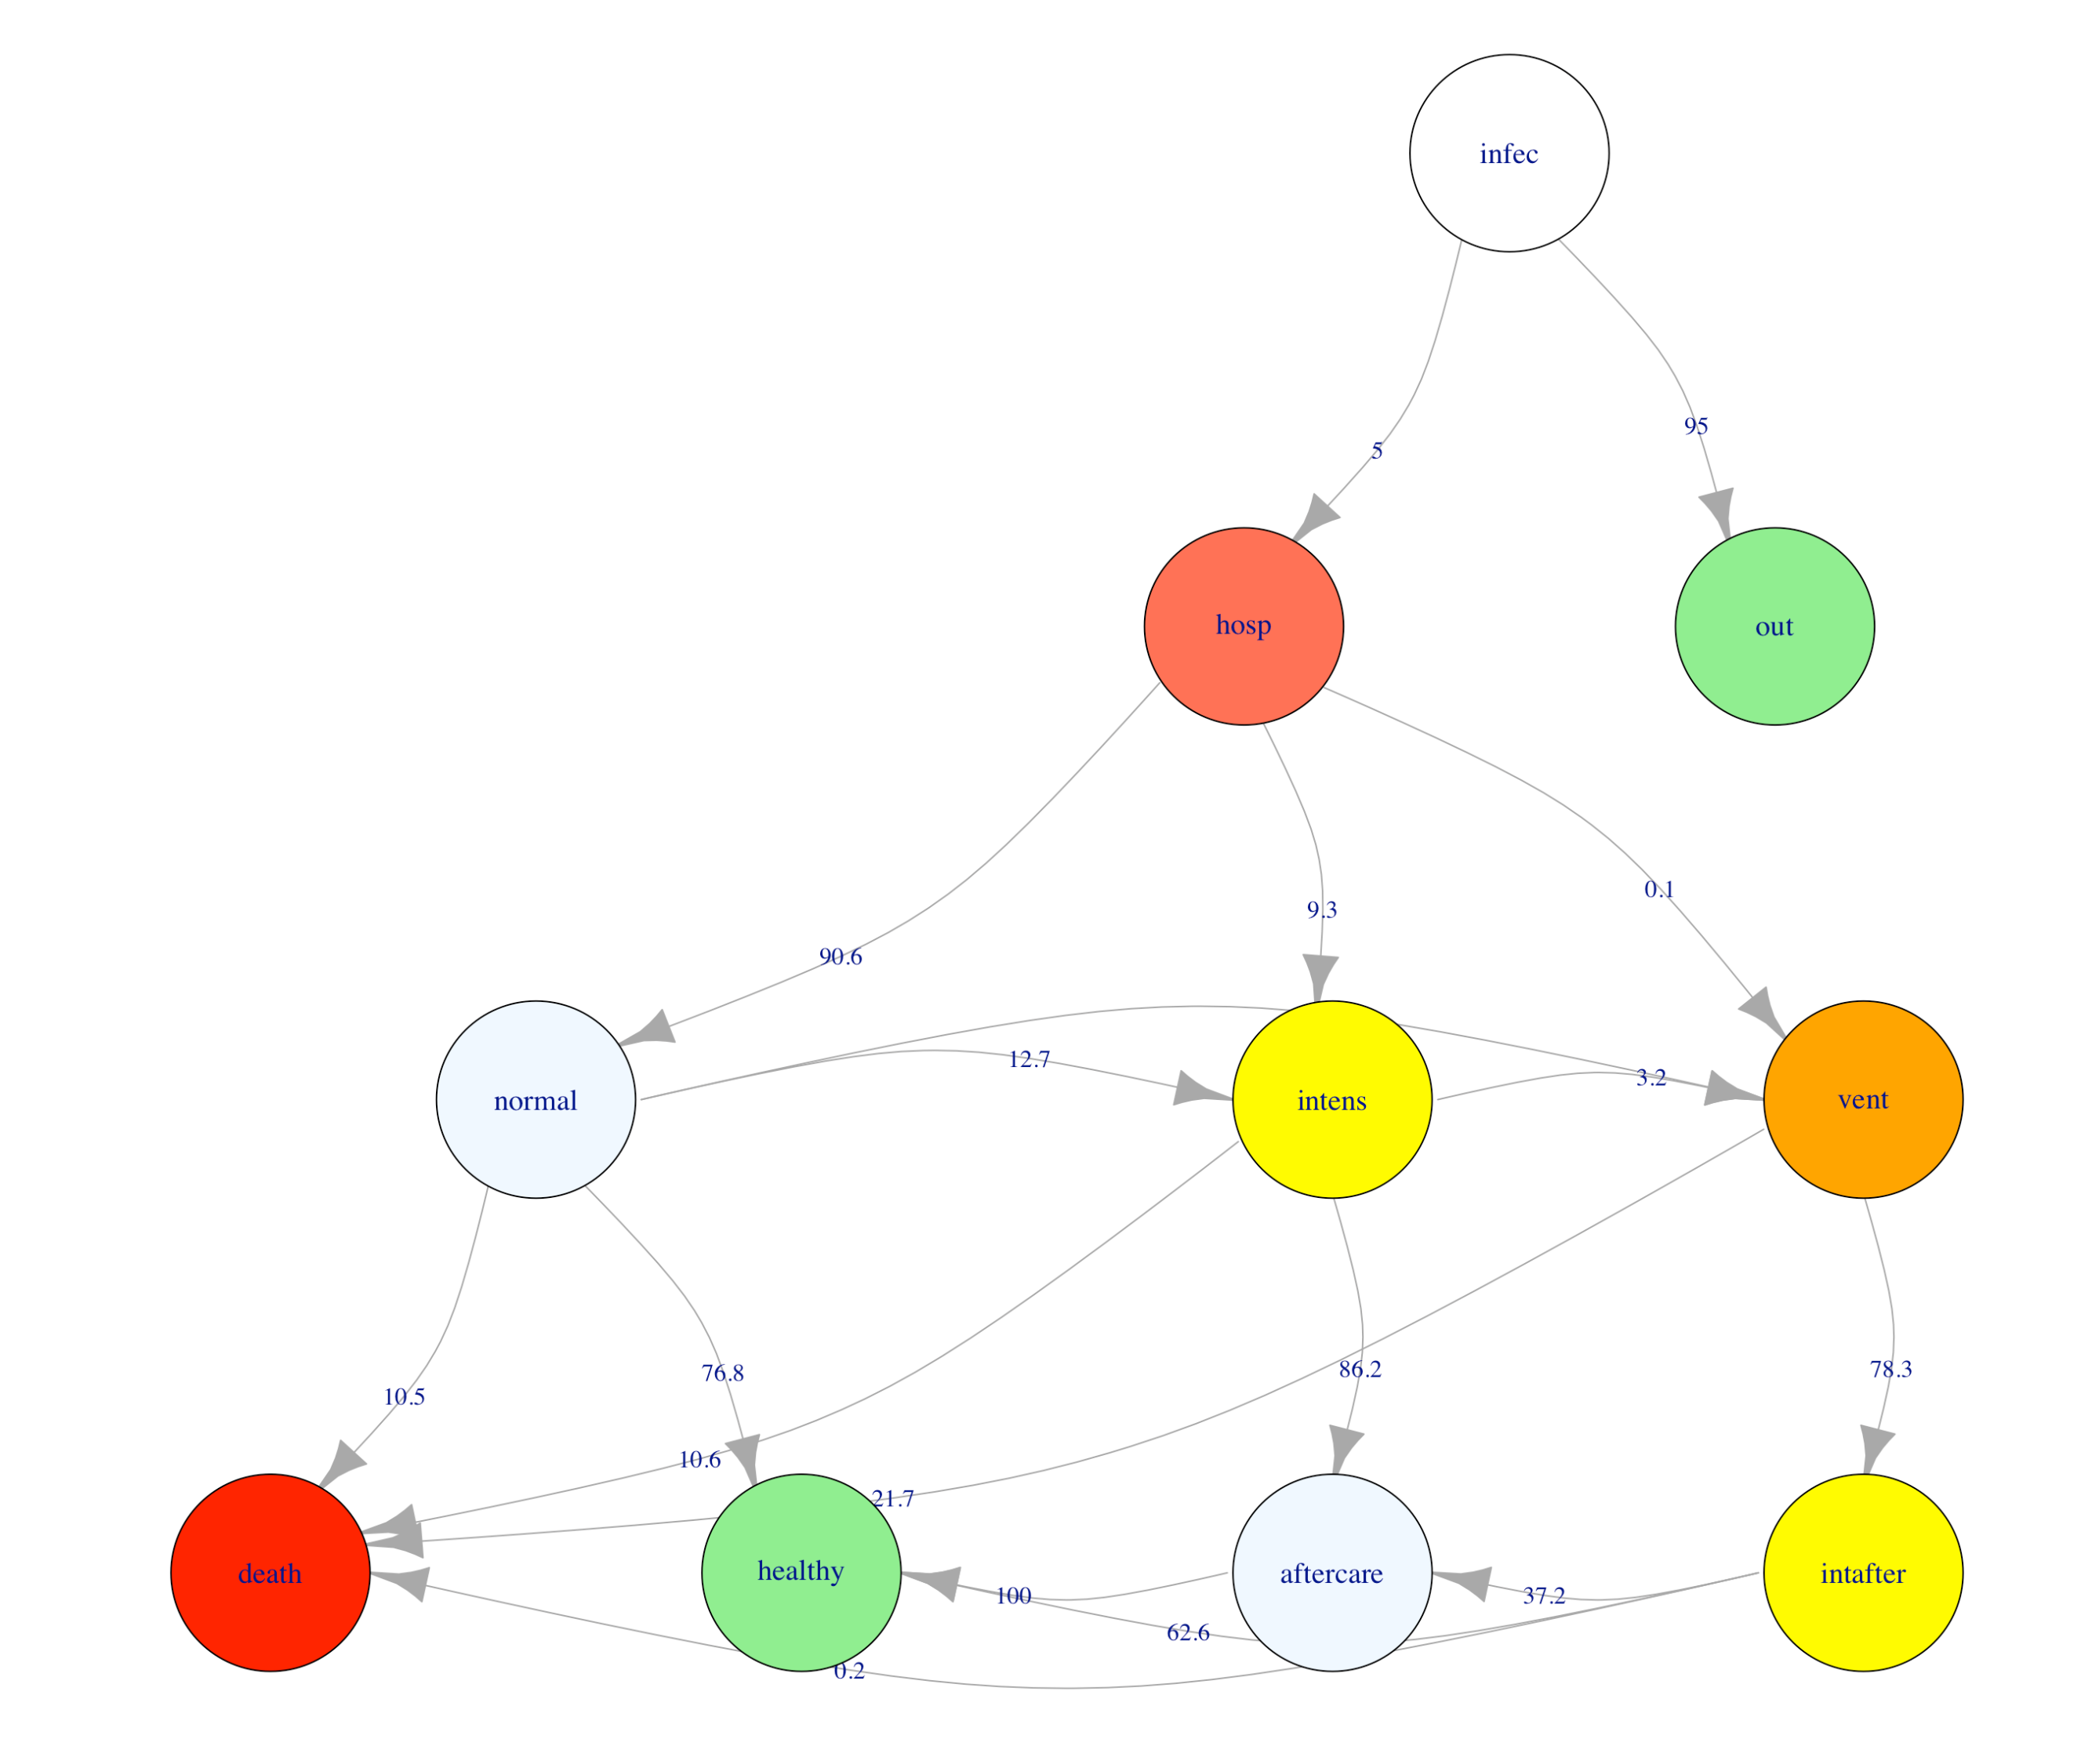
\includegraphics[width=0.75\linewidth]{prob.png}
    \caption{Full model of patient flows in a hospital. Nodes represent states ($S_i$). Edges represent state changes with associated probabilities ($p_{ij}$). The nodes are labeled as follows: \emph{Infec:}\/ Number of people tested positiv for Covid-19, published by RKI, 
\emph{out:}\/ Infected people not hospitalized, \emph{hosp:}\/ Hopitalized infected people, \emph{normal:}\/ Isolation ward, \emph{intens:}\/ Intensive care ward without invasive ventilation, \emph{vent:}\/ Intensive care ward with invasive ventilation, \emph{intafter:}\/ Intensive aftercare ward without invasive ventilation, \emph{aftercare:}\/ Aftercare isolation ward, \emph{healthy:}\/ Discharged as recovered, and \emph{death:}\/ Deceased.
This graph shows the core of \babsimhospital. This sets \babsimhospital apart from other simulators. It enables a detailed analysis of the underlying events. Upon request, it can be adapted to the individual circumstances of interested parties.}
\label{fig:prob}
\end{figure*}


For example, an infected patient (state $S_1$) goes to the hospital (state $S_2$) with probability $p_{12}$ after $d_{12}$ days. With probability $p_{17}$, she recovers (state $S_7$) after $d_{17}$ days. 
The probabilities of outgoing nodes sum to 1, e.g., $p_{17} = 1 - p_{12}$.
The modeling process includes four types of parameters: 
\begin{description}
\item[transition probabilities,] e.g., the probability that an infected individual has to go to the hospital,
\item[durations,] e.g., the time span until an infected individual goes to the hospital (in days), and
\item[distribution properties,] e.g., truncated and translated gamma distribution,
\item[risk factors] depending on demographic groups, e.g., age, gender. 
\end{description}


The "risk" attribute is an important factor for the duration and severity of a COVID-19 infection. 
Statistics show that the risk depends on the age and gender of the infected person. 
In our simulation, this risk is stored as an attribute of the patients. 
Every new patient is assigned a unique risk. 
We use an exponential function to model the relationship between the age of the person and their risk.
That means that older patients have a much higher probability of requiring an intensive bed or an intensive bed with ventilation than younger patients. 
In addition, men have a 50 percent higher risk than women. 



Proper tuning of these parameters is essential to obtain accurate predictions based on up-to-date and local data. 
The time-dependent changes require a frequent refitting of the model parameters to the current situation.
Thus, a daily parameter tuning procedure is run for each German region in order to provide an accurate prediction with \babsimhospital. 
An initial estimate for each of the given parameters was specified in cooperation with medical professionals. 
For example, the rate of successful treatments in Germany drastically changed between the first and the second wave of COVID-19 infections. 
Also, political decisions on national and local level can affect the situation significantly. 
While reducing the access to nursing homes might reduce infections in the high risk parts of the population, opening schools might cause many infections in the younger parts of the population. The optimization problem can be stated as follows:
the \babsimhospital simulator requires two input parameters:
\begin{compactenum}
\item $\vec{x}_t$, the model parameters
\item $\vec{u}_t$, the number of infections.
\end{compactenum}
Based on these two inputs, \babsimhospital estimates the required resources---in our case, the beds, \gls{ICU} beds,  and \gls{ICU} beds with ventilators.
The simulation output, i.e, the required resources on each day $t$ will be denoted as $\hat{\vec{y}}_t$, i.e., 
\begin{equation}\label{eq:haty}
\hat{y}_t = \left( \hat{R}_{\text{bed}}(t),   \hat{R}_{\text{icu}}(t), \hat{R}_{\text{vent}}(t) \right)
\end{equation}
Although the tool was designed to assist the German local authorities, it was already adapted and used for resource planing in hospitals in other countries.


\subsection{The Online-Version}\label{sec:online}
%%% TODO: Besser formulieren, mit Abbildung verknuepfen
See Fig.~\ref{fig:demo}

\begin{figure*}
    \centering
    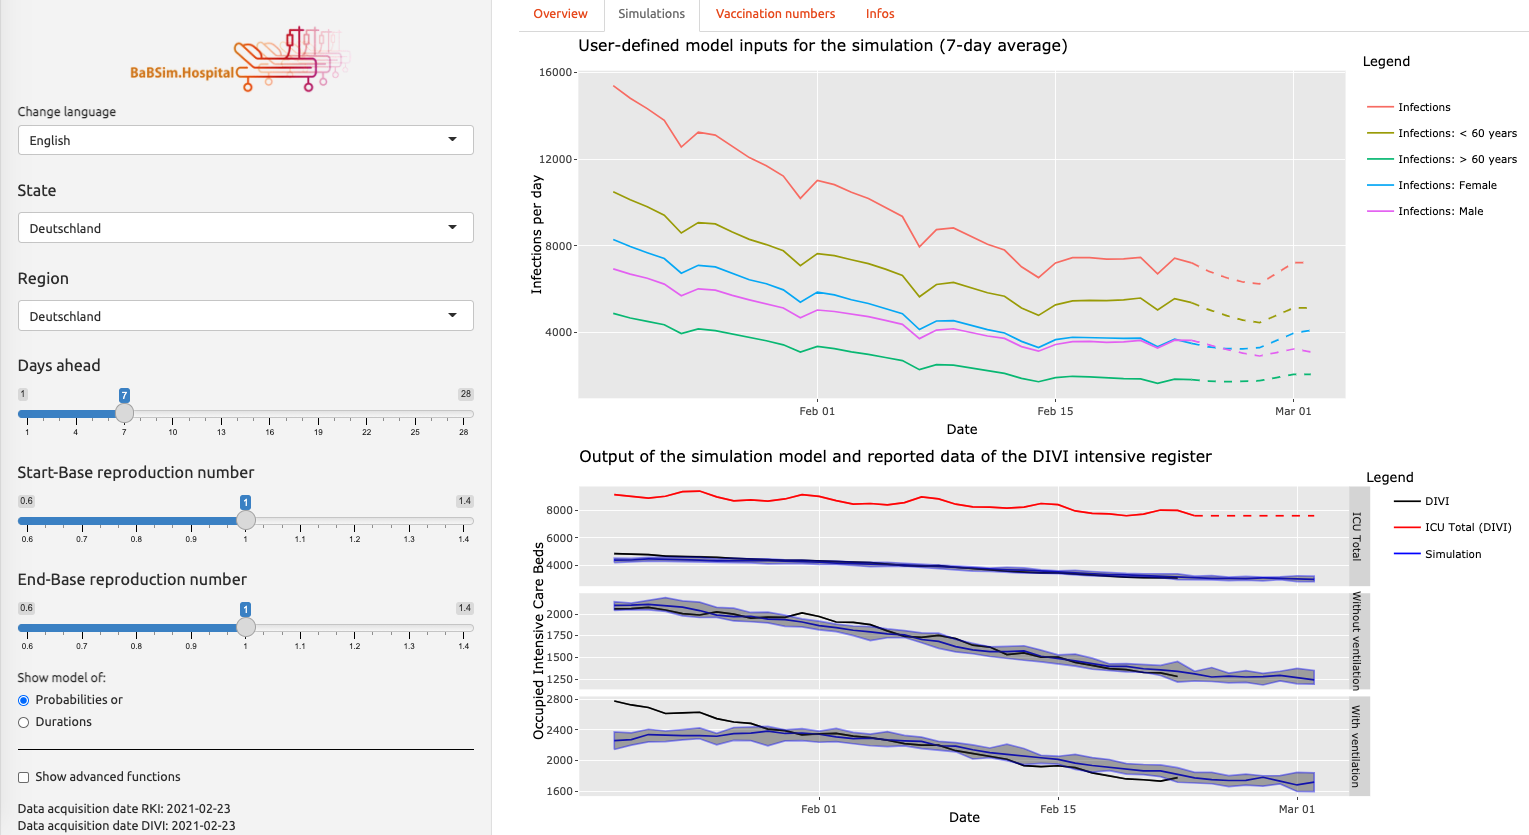
\includegraphics[width=\linewidth]{demoFR.png}
    \caption{Online version. }
\label{fig:demo}
\end{figure*}

\babsimhospital has the following advantages for crisis teams:
\begin{compactitem}
\item Comparison with your own local planning
\item Simulation of local events
\item Adaptation to your own situation
\item Simulation of any scenario (worst / best case)
\item Simulation of any pandemic scenario, considering the local situation
\item Standardized approach 
\end{compactitem}
Furthermore, it provides benefits for medical professionals, e.g.,
\begin{compactitem}
\item Analysis of the pandemic at local, regional, state and federal level
\item Consideration of special risk groups
\item Validation of the length of stay
\item Validation of the probabilities
\end{compactitem}

Last, but not least, administration and management can benefit from \babsimhospital, because
\begin{compactitem}
\item Assessment of the situation of individual hospitals taking local events into account
\item Consideration of relevant resources: beds, ventilators, rooms, protective clothing
\item Personnel planning: medical and nursing staff
\end{compactitem}

\subsection{Open Source}
\babsimhospital is open source. It is programmed in the R language and environment for statistical computing and graphics and freely available, see~\cite{bart20t}.


\section{Optimization}\label{sec:optim}
Optimization tries to improve the \gls{RMSE} as defined in Eq.~\ref{eq:rmse}.
After the optimization-via-simulation problem is defined, this section describes the current state in optimization and discusses the selection of a suitable optimizer. 

\subsection{Optimization Problem}
Based on the simulation results, optimization runs can be performed to improve parameter settings proposed by the experts. 
The \gls{RMSE} as shown in Eq.~\ref{eq:rmse}, is used to measure the error of the simulator.
We formulate the \emph{minimization} problem:
\begin{equation}\label{eq:rmse}
  \min 
  \sum_{k\in\{\text{bed},\text{icu},\text{vent}\}}
    w_k  \sqrt{\frac{1}{T} \sum_{t=1}^T \left(R_k(t) - \hat{R}_k(t)\right)^2}
\end{equation}
Here, $T$ denotes the number of days simulated and $k$ the three different bed categories.
Since the different bed types are not equally important a weighted average of the \gls{RMSE} for each bed category is used as the final error measure.
A detailed description can be found in~\citep{Bart20j}.

The extensive amount of data that the tool has to process combined with the high dimensionality of the problem, and the required accuracy make simplifying the modeling process to improve performance a big challenge.
The limited time available for each optimization run requires the use of efficient algorithms.
To resolve that problem, a number of different optimization-via-simulation techniques can be used. 
These will be covered in the following.

\subsection{Standard Optimizers}
First, the applicability of standard optimization algorithms, e.g., BOBYQA~\citep{Powe09a}, CMA-ES~\citep{Hans06a}, Simulated Annealing~\citep{vanL87a}, was tested. Pre-experimental results revealed that these optimizers were not able to find an improved parameter configurations under the hard time constraints posed by this problem. 

\subsection{Parallelizing and  Combining Global with Local Optimizers}\label{sec:comb}
\citet{Good18b} presented during last years' GECCO \gls{ECiP} track approaches that implement combinations of global and local search methods with a special focus on black-box optimizers.
He discussed optimization strategies that combine different optimization methods. 
For example, the commercial software HEEDS contains a unique search strategy called \gls{SHERPA}~\citep{Good08a}.
During a single search, \gls{SHERPA} uses multiple search methods in parallel.
This approach takes advantage of the strengths of each method, and reduces a methods’ participation in the search if/when it is determined to be ineffective.
However, because \gls{SHERPA} is a commercial software, it was not applicable to our problem.

\subsection{Massively Parallel Single-Iteration Optimizers}\label{sec:parallel}
During the last years the availability of parallel computation increased significantly. 
Even personal computers are equipped with multi-core processors and allow simple parallel optimizations. Recent approaches take parallelization to the extreme: why not use several thousands, or millions of processors in parallel for a so-called \emph{one-shot} optimization run?
In one-shot optimization, aka single-iteration evolution or fully-parallel optimization, the user selects a population, evaluates it, and has to base all future decisions only on the quality of these points.
In a recent work, \citet{Cauw20a} analyzed the setting in which an optimal solution is chosen at random from a Gaussian distribution.
They could prove that, unlike one might expect, it is better to sample only one (namely, the center of the distribution) rather than sampling $n$ times from the same Gaussian distribution.

Fully-parallel optimization was also proposed for hyperparameter search~\citep{Cauw20a}.
The authors  demonstrated that it can be be more effective than random and grid search and that performance improvement can be obtained in a wide range of expensive artificial intelligence tasks.
Furthermore, \citet{Rena20a} discuss the sensitivity of the fitness landscape analysis to fully-parallel optimization sampling strategies, which is also of great relevance in this context, because the sampling strategy is crucial in fully-parallel optimization.
The fully-parallel optimization approach is used in industry by companies like Facebook, that have large server farms at their disposal.
It is considered as the only possible solution if optimization has to be done under very hard time constraints. 
However, this approach was not applicable for our optimization, because we only have a few hundred CPU cores available.

\subsection{Response Surface Methodology and Surrogate Model-based Optimizers}\label{sec:rsm}
\gls{RSM} is a collection of statistical and mathematical tools useful for developing, improving, and optimizing processes~\citep{Myers2016}. 
Applications historically come from industry and manufacturing, 
However, in many settings, their intended application is too local. Moreover, \gls{RSM} is ``too hands-on''.
Because computational power is available in every real-world optimization scenario, 
it might be useful to automate, i.e., to remove humans from the loop and set the computer running on the optimization in order to maximize computing throughput, or minimize idle time. 
Therefore, new response surface methodologies were developed in the last decades~\citep{Gram20a}.
 
 One prominent representative in very budget-restricted environments is \gls{SMBO}~\citep{Jin11a}.
In \gls{SMBO}, a data-driven surrogate is fitted to only a few initial sample points on the expensive to evaluate objective function. 
The fitted model is (compared to the real objective function) computationally cheap to evaluate.
Thus, promising new candidate solutions can be proposed by running an extensive optimization on the model.
The search on the model is guided by a so-called infill criterion or often also acquisition function.
The function assigns a quantitative quality, usually based on the models prediction and uncertainty, to a given candidate.
The best candidate proposed by the model is evaluated on the expensive objective function and a new model is fitted including the new data point.
This process is iterated until the budget of expensive evaluations is depleted or some other stopping criterion is met. More in-depth explanations of model-based optimization and its applications can be found in~\citet{Quei05a, EGOB02, Jin19a}.

Only \gls{SMBO} approaches produced good results. 
Therefore, the \gls{SPOT} algorithm was chosen~\citep{Bart17parxiv}.
To accelerate the \gls{SPOT}, simulations were run in parallel.
Besides robust and relatively fast optimizations, \gls{SPOT} provides an additional advantage: surrogate models used by the optimizer can be used (``recycled'') for a sensitivity analysis. 

\section{Adaptation of the Search Boundaries}\label{sec:adaptation}
\subsection{Germany}



\subsection{United Kingdom}
Compared to Germany, there is only a small number of ICU beds with ventilation in the UK.
Therefore, patients are treated differently: the percentage of patients sent to \gls{ICU} with ventilation should be reduced.
We will adopt the boundaries of the search space (constraints) to reduce the probabilities.

\subsubsection{First Adaptation: Reducing Probabilities}
Table~\ref{tab:para} presents an overview of the parameter ranges of the 29 parameters used in the \babsimhospital simulation model.

% latex table generated in R 4.0.4 by xtable 1.8-4 package
% Tue Feb 23 15:02:12 2021
\begin{table*}[ht]\label{tab:para}
\caption{Default and adapted parameter ranges.}
\centering
\begin{tabular}{llrrrrr}
  \hline
Variable & Name & default & minUK & maxUK & minDE & MaxDE \\ 
  \hline
$x_1$&  AmntDaysInfectedToHospital & 9.50 & 6.00 & 14.00 & 6.00 & 14.00 \\ 
$x_2$&   AmntDaysNormalToHealthy & 10.00 & 7.00 & 13.00 & 7.00 & 13.00 \\ 
$x_3$&   AmntDaysNormalToIntensive & 5.00 & 3.00 & 7.00 & 3.00 & 7.00 \\ 
$x_4$&  AmntDaysNormalToVentilation & 3.63 & 3.00 & 9.00 & 3.00 & 9.00 \\ 
$x_5$&   AmntDaysNormalToDeath & 5.00 & 3.00 & 7.00 & 3.00 & 7.00 \\ 
$ \mathbf{x_6}$&   \textbf{AmntDaysIntensiveToAftercare} & $\mathbf{7.00}$ & $\mathbf{10.00}$ & $\mathbf{18.00}$ & $\mathbf{5.00}$ & $\mathbf{9.00}$ \\ 
$\mathbf{x_7}$ &   \textbf{AmntDaysIntensiveToVentilation} & $\mathbf{4.00}$ & $\mathbf{6.00}$ & $\mathbf{10.00}$ & $\mathbf{3.00}$ & $\mathbf{5.00}$ \\ 
$\mathbf{x_8}$&   \textbf{AmntDaysIntensiveToDeath} & $\mathbf{5.00}$ & $\mathbf{6.00}$ & $\mathbf{14.00}$ & $\mathbf{3.00}$  & $\mathbf{7.00}$ \\ 
$x_9$&   AmntDaysVentilationToIntensiveAfter & 30.00 & 25.00 & 35.00 & 25.00 & 35.00 \\ 
$x_{10}$&   AmntDaysVentilationToDeath & 20.00 & 17.00 & 25.00 & 17.00 & 25.00 \\ 
$x_{11}$&   AmntDaysIntensiveAfterToAftercare & 3.00 & 2.00 & 5.00 & 2.00 & 5.00 \\ 
$x_{12}$&   AmntDaysIntensiveAfterToDeath & 4.00 & 1.00 & 7.00 & 1.00 & 7.00 \\ 
$x_{13}$&   GammaShapeParameter & 1.00 & 0.25 & 2.00 & 0.25 & 2.00 \\ 
$x_{14}$&   FactorPatientsInfectedToHospital & 0.10 & 0.05 & 0.15 & 0.05 & 0.15 \\ 
$x_{15}$&   FactorPatientsHospitalToIntensive & 0.09 & 0.07 & 0.11 & 0.07 & 0.11 \\ 
$ \mathbf{x_{16}}$ & \textbf{FactorPatientsHospitalToVentilation} & $ \mathbf{0.01}$ & $ \mathbf{0.001}$ & $ \mathbf{0.002} $& $ \mathbf{0.01}$ & $ \mathbf{0.02}$ \\ 
$x_{17}$&   FactorPatientsNormalToIntensive & 0.10 & 0.07 & 0.13 & 0.07 & 0.13 \\ 
$\mathbf{x_{18}}$&   \textbf{FactorPatientsNormalToVentilation} & $\mathbf{0.00}$ & $\mathbf{1e-05}$ & $\mathbf{0.0002}$ & $\mathbf{1e-04}$ & $\mathbf{ 0.0020}$ \\ 
$x_{19}$&   FactorPatientsNormalToDeath & 0.10 & 0.08 & 0.12 & 0.08 & 0.12 \\ 
$\mathbf{x_{20}}$&   \textbf{FactorPatientsIntensiveToVentilation} & $\mathbf{0.30}$ & $\mathbf{0.03}$ & $\mathbf{0.03}$ & $\mathbf{0.25}$ & $\mathbf{0.35}$ \\ 
$x_{21}$&   FactorPatientsIntensiveToDeath & 0.10 & 0.08 & 0.12 & 0.08 & 0.12 \\ 
$x_{22}$&   FactorPatientsVentilationToIntensiveAfter & 0.70 & 0.50 & 0.90 & 0.50 & 0.90 \\ 
$x_{23}$&   FactorPatientsIntensiveAfterToDeath & 0.00 & 0.00 & 0.01 & 0.00 & 0.01 \\ 
$x_{24}$&   AmntDaysAftercareToHealthy & 3.00 & 2.00 & 4.00 & 2.00 & 4.00 \\ 
$x_{25}$&   RiskFactorA & 0.02 & 0.00 & 1.10 & 0.00 & 1.10 \\ 
$x_{26}$&   RiskFactorB & 0.01 & 0.00 & 0.06 & 0.00 & 0.06 \\ 
$x_{27}$&   RiskMale & 1.50 & 1.00 & 2.00 & 1.00 & 2.00 \\ 
$x_{28}$&   AmntDaysIntensiveAfterToHealthy & 3.00 & 2.00 & 5.00 & 2.00 & 5.00 \\ 
$x_{29}$&   FactorPatientsIntensiveAfterToHealthy & 0.67 & 0.50 & 0.75 & 0.50 & 0.75 \\ 
   \hline
\end{tabular}
\end{table*}


To implement the different setting, we modified the parameter boundaries as follows: the ICU with ventilation node has three incoming edges (hospital to icu vent, normal station to icu vent, and icu station to icu vent).
By introducing a reduction factor, say  $c_1 \in \mathbb{R_+}$, that simply multiplies the default probabilities of patients reaching the icu ventilated node, we were able to redirect patients to other bed categories. 
Choosing a value of $c_1=0.1$ results in improved simulation outputs. Please note that $c_1$ does not directly affect the probabilities, it modifies the search boundaries (constraints) of the optimizer.

Simulation results of the ventilated icu beds were significantly improved (both: numerical RMSE and visual inspection as can be seen in Fig.~\ref{fig:optimized}.


\begin{compactitem} 
\item[$x_{16}$:] The range of the parameter \texttt{Factor\-Patients\-Hospital\-To\-Ventilation}  was reduced from $[0.01; 0.02]$ to $[5.0e-04; 0.0020]$. 
\item[$x_{18}$:] The range of the parameter \texttt{Factor\-Patients\-Normal\-To\-Ventilation} was reduced from $[0.1; 0.2]$ to $[0.01; 0.02]$. 
\item[$x_{20}$:] The range of the parameter \texttt{Factor\-Patients\-Intensive\-To\-Ventilation} was reduced from $[0.1; 0.2]$ to $[0.01; 0.02]$. 
\end{compactitem}


\subsubsection{Second Adaptation: Increasing Durations}

However, even if the ventilated icu bed usage was improved (bed category III), the simulation of the second bed category is not satisfying. We under estimate the number of icu beds.
To fix this problem, we modified the duration of patients in icu beds: the search intervals of theses parameters were increased. Therefore, a second factor, say $c_2 \in \mathbb{R}_+$ was introduced to multiply the corresponding durations. A value of $c_2 = 2.0$ was chosen for our experiments.



\begin{compactitem} 
\item[$x_{6}$:] The range of the parameter \texttt{AmntDays\-Intensive\-To\-Aftercare} was increased from $[5;9]$ to $[10;18]$ days.
\item[$x_{7}$:] The parameter \texttt{AmntDays\-Intensive\-To\-Ventilation} was increased from $[3;5]$ to $[6;10]$ days.
\item[$x_{8}$:] The parameter \texttt{AmntDays\-Intensive\-To\-Death} was increased from $[3;7]$ to $[6;14]$ days.
\end{compactitem}


\section{Results}\label{sec:results}
\begin{figure*}
  \centering
   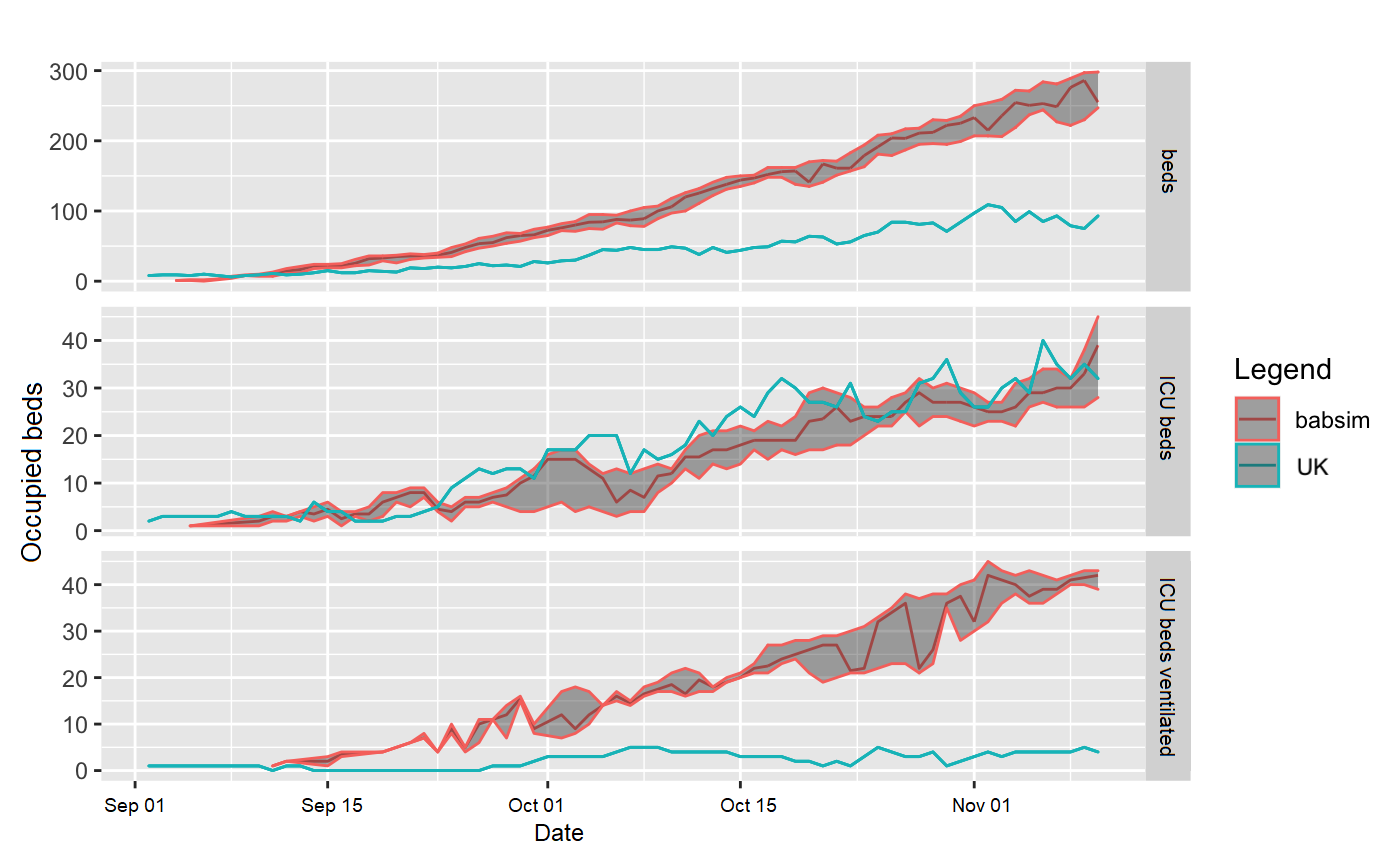
\includegraphics[width=0.7\textwidth]{default.png}
  \caption{Real data compared to results from the \babsimhospital simulation with default parameters. Large residuals (errors), especially for normal bed and icu beds with ventilation can be observed.
   \babsimhospital uses default parameter sets. These are based on domain knowledge (recommendations from doctors) from Germany. }
\label{fig:default}
\end{figure*}
\begin{figure*}
    \centering
    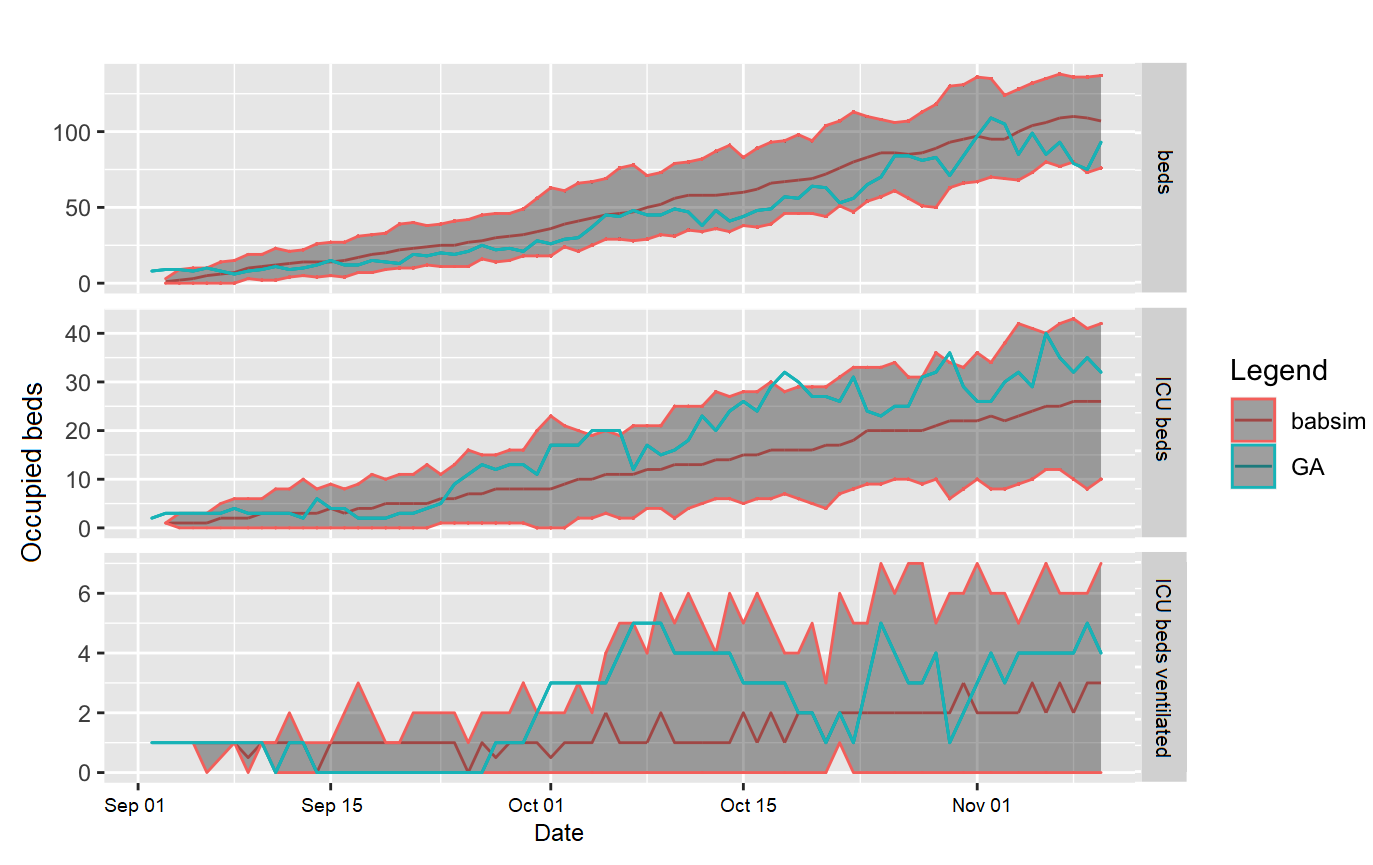
\includegraphics[width=0.7\textwidth]{optimized01.png}
    \caption{Real data compared to results from the \babsimhospital simulation with optimized parameters. The comparison with the results from Fig.~\ref{fig:default} shows a significant improvement. However, considering the regular \gls{ICU} beds (category II) there is still a difference between the real data and the simulated data. Therefore, a second adaption was necessary.
  }
\label{fig:optimized01}
\end{figure*}
\begin{figure*}
    \centering
    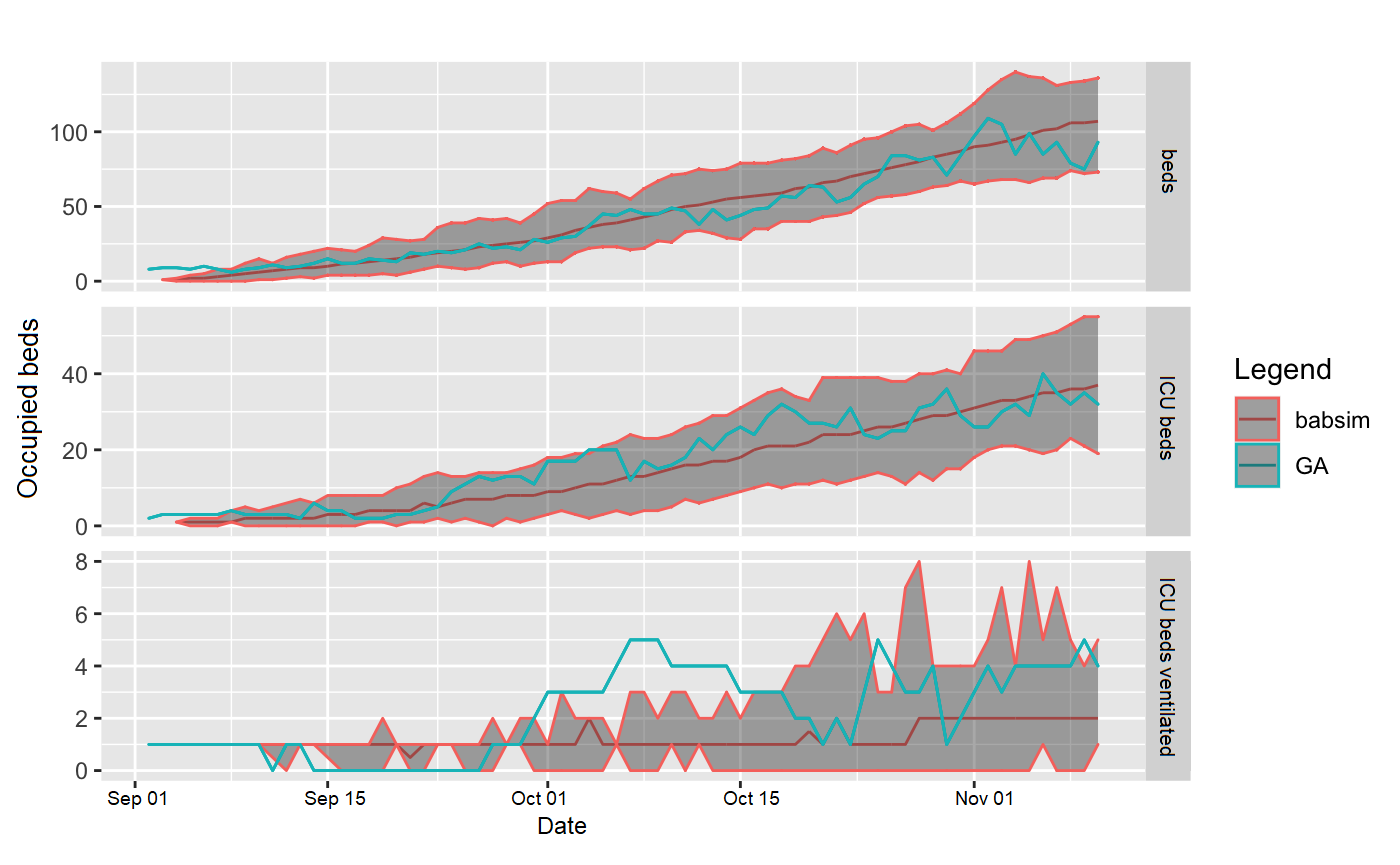
\includegraphics[width=0.7\textwidth]{optimized.png}
    \caption{Real data compared to results from the \babsimhospital simulation with optimized parameters. The comparison with the results from Fig.~\ref{fig:default} shows a significant improvement. Residuals are much smaller,
    because the simulation model parameters were adapted to the situation in UK hospitals. Additionally, simulation results for category II beds is improved.  
  }
\label{fig:optimized}
\end{figure*}

The adaptation of the parameter bounds based on domain knowledge results in a significant reduction of the \gls{RMSE}, which was defined in  Eq.~\ref{eq:rmse}. 
Using the default \babsimhospital parameter boundaries, which were based on the situation in Germany, the simulation error is $\epsilon_0 = 184.10$.
The first adaptation, which reduces the percentage of patients treated in \gls{ICU} beds with ventilation, results in an simulation error $\epsilon_1 =  55.67$, whereas the second adaption, which increases the duration patients in \gls{ICU} bed results in a further reduction of the simulation error to $\epsilon_2 = 28.10$. In summary, the adaptation has been shown to reduce simulation errors by nearly 70\%.

Figures~\ref{fig:default}, \ref{fig:optimized01}, and \ref{fig:optimized} clearly visualize the improvements.


\section{Discussion and Outlook}\label{sec:discussion}
The high dimension and computational expense of the \babsimhospital simulator 
poses a challenging optimization task. 
Solving this task for many regions in Germany under very different local circumstances requires 
efficient solutions to cope with the further growing infection numbers and thus also growing simulation run times. 
This article presents a holistic approach to solve this challenging problem. 
It reports experiences from a one-year project with several stakeholders. 
From the Questions posed in Section~\ref{sec:intro} we would like to answer (Q-1) to (Q-3) directly.
\begin{compactenum}[(Q-1)]
\item How to automate data collection and curation?
The system is running fully automatically for several months.
It allows processing  the \gls{RKI} data set, which consists of more than 
750,000 observations of 18 variables, which are updated daily and are automatically integrated into \babsimhospital simulator. 
The \gls{CICD} approach minimizes human interaction, so that simulations and optimizations are
started automatically after the data is downloaded.
\item How to select a suitable simulation model?
The \gls{DES} delivers valid results and enables predictions, which are valuable for capacity planning in hospitals.
The \gls{simmer} software presents a good basis for implementation and was able to handle more than half a million data (infections) under very limited time constraints. 
\item How to find an optimization algorithm that is able to solve noisy, dynamic, high-dimensional real-world problems?
Using "out-of-the-box" optimizers did not work, because the problem is too noisy and high-dimensional.
Applying model-based optimizers to this simulation problem provided good results but also slightly increased the computational burden due to the runtime of the model-based optimizer. 
Using the estimated parameter importances from the sensitivity analysis indicated that running the model-based optimizer with fewer parameters is possible without a significant quality loss. 
Removing parameters from the model-based optimization loop can drastically decrease the optimizers runtime. 
\end{compactenum}
\subsubsection*{Conclusion and Outlook}
The \babsimhospital simulator can be used as attractive simulation and optimization benchmark example. Its source code is open source. 



\bibliographystyle{ACM-Reference-Format}
\bibliography{sample-base}
\end{document}

\endinput


\section{Introduction}
This document is a model and instructions for \LaTeX.
Please observe the conference page limits. 

\section{Ease of Use}

\subsection{Maintaining the Integrity of the Specifications}

The IEEEtran class file is used to format your paper and style the text. All margins, 
column widths, line spaces, and text fonts are prescribed; please do not 
alter them. You may note peculiarities. For example, the head margin
measures proportionately more than is customary. This measurement 
and others are deliberate, using specifications that anticipate your paper 
as one part of the entire proceedings, and not as an independent document. 
Please do not revise any of the current designations.

\section{Prepare Your Paper Before Styling}
Before you begin to format your paper, first write and save the content as a 
separate text file. Complete all content and organizational editing before 
formatting. Please note sections \ref{AA}--\ref{SCM} below for more information on 
proofreading, spelling and grammar.

Keep your text and graphic files separate until after the text has been 
formatted and styled. Do not number text heads---{\LaTeX} will do that 
for you.

\subsection{Abbreviations and Acronyms}\label{AA}
Define abbreviations and acronyms the first time they are used in the text, 
even after they have been defined in the abstract. Abbreviations such as 
IEEE, SI, MKS, CGS, ac, dc, and rms do not have to be defined. Do not use 
abbreviations in the title or heads unless they are unavoidable.

\subsection{Units}
\begin{itemize}
\item Use either SI (MKS) or CGS as primary units. (SI units are encouraged.) English units may be used as secondary units (in parentheses). An exception would be the use of English units as identifiers in trade, such as ``3.5-inch disk drive''.
\item Avoid combining SI and CGS units, such as current in amperes and magnetic field in oersteds. This often leads to confusion because equations do not balance dimensionally. If you must use mixed units, clearly state the units for each quantity that you use in an equation.
\item Do not mix complete spellings and abbreviations of units: ``Wb/m\textsuperscript{2}'' or ``webers per square meter'', not ``webers/m\textsuperscript{2}''. Spell out units when they appear in text: ``. . . a few henries'', not ``. . . a few H''.
\item Use a zero before decimal points: ``0.25'', not ``.25''. Use ``cm\textsuperscript{3}'', not ``cc''.)
\end{itemize}

\subsection{Equations}
Number equations consecutively. To make your 
equations more compact, you may use the solidus (~/~), the exp function, or 
appropriate exponents. Italicize Roman symbols for quantities and variables, 
but not Greek symbols. Use a long dash rather than a hyphen for a minus 
sign. Punctuate equations with commas or periods when they are part of a 
sentence, as in:
\begin{equation}
a+b=\gamma\label{eq}
\end{equation}

Be sure that the 
symbols in your equation have been defined before or immediately following 
the equation. Use ``\eqref{eq}'', not ``Eq.~\eqref{eq}'' or ``equation \eqref{eq}'', except at 
the beginning of a sentence: ``Equation \eqref{eq} is . . .''

\subsection{\LaTeX-Specific Advice}

Please use ``soft'' (e.g., \verb|\eqref{Eq}|) cross references instead
of ``hard'' references (e.g., \verb|(1)|). That will make it possible
to combine sections, add equations, or change the order of figures or
citations without having to go through the file line by line.

Please don't use the \verb|{eqnarray}| equation environment. Use
\verb|{align}| or \verb|{IEEEeqnarray}| instead. The \verb|{eqnarray}|
environment leaves unsightly spaces around relation symbols.

Please note that the \verb|{subequations}| environment in {\LaTeX}
will increment the main equation counter even when there are no
equation numbers displayed. If you forget that, you might write an
article in which the equation numbers skip from (17) to (20), causing
the copy editors to wonder if you've discovered a new method of
counting.

{\BibTeX} does not work by magic. It doesn't get the bibliographic
data from thin air but from .bib files. If you use {\BibTeX} to produce a
bibliography you must send the .bib files. 

{\LaTeX} can't read your mind. If you assign the same label to a
subsubsection and a table, you might find that Table I has been cross
referenced as Table IV-B3. 

{\LaTeX} does not have precognitive abilities. If you put a
\verb|\label| command before the command that updates the counter it's
supposed to be using, the label will pick up the last counter to be
cross referenced instead. In particular, a \verb|\label| command
should not go before the caption of a figure or a table.

Do not use \verb|\nonumber| inside the \verb|{array}| environment. It
will not stop equation numbers inside \verb|{array}| (there won't be
any anyway) and it might stop a wanted equation number in the
surrounding equation.

\subsection{Some Common Mistakes}\label{SCM}
\begin{itemize}
\item The word ``data'' is plural, not singular.
\item The subscript for the permeability of vacuum $\mu_{0}$, and other common scientific constants, is zero with subscript formatting, not a lowercase letter ``o''.
\item In American English, commas, semicolons, periods, question and exclamation marks are located within quotation marks only when a complete thought or name is cited, such as a title or full quotation. When quotation marks are used, instead of a bold or italic typeface, to highlight a word or phrase, punctuation should appear outside of the quotation marks. A parenthetical phrase or statement at the end of a sentence is punctuated outside of the closing parenthesis (like this). (A parenthetical sentence is punctuated within the parentheses.)
\item A graph within a graph is an ``inset'', not an ``insert''. The word alternatively is preferred to the word ``alternately'' (unless you really mean something that alternates).
\item Do not use the word ``essentially'' to mean ``approximately'' or ``effectively''.
\item In your paper title, if the words ``that uses'' can accurately replace the word ``using'', capitalize the ``u''; if not, keep using lower-cased.
\item Be aware of the different meanings of the homophones ``affect'' and ``effect'', ``complement'' and ``compliment'', ``discreet'' and ``discrete'', ``principal'' and ``principle''.
\item Do not confuse ``imply'' and ``infer''.
\item The prefix ``non'' is not a word; it should be joined to the word it modifies, usually without a hyphen.
\item There is no period after the ``et'' in the Latin abbreviation ``et al.''.
\item The abbreviation ``i.e.'' means ``that is'', and the abbreviation ``e.g.'' means ``for example''.
\end{itemize}
An excellent style manual for science writers is \cite{b7}.

\subsection{Authors and Affiliations}
\textbf{The class file is designed for, but not limited to, six authors.} A 
minimum of one author is required for all conference articles. Author names 
should be listed starting from left to right and then moving down to the 
next line. This is the author sequence that will be used in future citations 
and by indexing services. Names should not be listed in columns nor group by 
affiliation. Please keep your affiliations as succinct as possible (for 
example, do not differentiate among departments of the same organization).

\subsection{Identify the Headings}
Headings, or heads, are organizational devices that guide the reader through 
your paper. There are two types: component heads and text heads.

Component heads identify the different components of your paper and are not 
topically subordinate to each other. Examples include Acknowledgments and 
References and, for these, the correct style to use is ``Heading 5''. Use 
``figure caption'' for your Figure captions, and ``table head'' for your 
table title. Run-in heads, such as ``Abstract'', will require you to apply a 
style (in this case, italic) in addition to the style provided by the drop 
down menu to differentiate the head from the text.

Text heads organize the topics on a relational, hierarchical basis. For 
example, the paper title is the primary text head because all subsequent 
material relates and elaborates on this one topic. If there are two or more 
sub-topics, the next level head (uppercase Roman numerals) should be used 
and, conversely, if there are not at least two sub-topics, then no subheads 
should be introduced.

\subsection{Figures and Tables}
\paragraph{Positioning Figures and Tables} Place figures and tables at the top and 
bottom of columns. Avoid placing them in the middle of columns. Large 
figures and tables may span across both columns. Figure captions should be 
below the figures; table heads should appear above the tables. Insert 
figures and tables after they are cited in the text. Use the abbreviation 
``Fig.~\ref{fig}'', even at the beginning of a sentence.

\begin{table}[htbp]
\caption{Table Type Styles}
\begin{center}
\begin{tabular}{|c|c|c|c|}
\hline
\textbf{Table}&\multicolumn{3}{|c|}{\textbf{Table Column Head}} \\
\cline{2-4} 
\textbf{Head} & \textbf{\textit{Table column subhead}}& \textbf{\textit{Subhead}}& \textbf{\textit{Subhead}} \\
\hline
copy& More table copy$^{\mathrm{a}}$& &  \\
\hline
\multicolumn{4}{l}{$^{\mathrm{a}}$Sample of a Table footnote.}
\end{tabular}
\label{tab1}
\end{center}
\end{table}

\begin{figure}[htbp]
\centerline{
\includegraphics{fig1.png}}
\caption{Example of a figure caption.}
\label{fig}
\end{figure}

Figure Labels: Use 8 point Times New Roman for Figure labels. Use words 
rather than symbols or abbreviations when writing Figure axis labels to 
avoid confusing the reader. As an example, write the quantity 
``Magnetization'', or ``Magnetization, M'', not just ``M''. If including 
units in the label, present them within parentheses. Do not label axes only 
with units. In the example, write ``Magnetization (A/m)'' or ``Magnetization 
\{A[m(1)]\}'', not just ``A/m''. Do not label axes with a ratio of 
quantities and units. For example, write ``Temperature (K)'', not 
``Temperature/K''.

\section*{Acknowledgment}

The preferred spelling of the word ``acknowledgment'' in America is without 
an ``e'' after the ``g''. Avoid the stilted expression ``one of us (R. B. 
G.) thanks $\ldots$''. Instead, try ``R. B. G. thanks$\ldots$''. Put sponsor 
acknowledgments in the unnumbered footnote on the first page.

\section*{References}

Please number citations consecutively within brackets \cite{b1}. The 
sentence punctuation follows the bracket \cite{b2}. Refer simply to the reference 
number, as in \cite{b3}---do not use ``Ref. \cite{b3}'' or ``reference \cite{b3}'' except at 
the beginning of a sentence: ``Reference \cite{b3} was the first $\ldots$''

Number footnotes separately in superscripts. Place the actual footnote at 
the bottom of the column in which it was cited. Do not put footnotes in the 
abstract or reference list. Use letters for table footnotes.

Unless there are six authors or more give all authors' names; do not use 
``et al.''. Papers that have not been published, even if they have been 
submitted for publication, should be cited as ``unpublished'' \cite{b4}. Papers 
that have been accepted for publication should be cited as ``in press'' \cite{b5}. 
Capitalize only the first word in a paper title, except for proper nouns and 
element symbols.

For papers published in translation journals, please give the English 
citation first, followed by the original foreign-language citation \cite{b6}.

\begin{thebibliography}{00}
\bibitem{b1} G. Eason, B. Noble, and I. N. Sneddon, ``On certain integrals of Lipschitz-Hankel type involving products of Bessel functions,'' Phil. Trans. Roy. Soc. London, vol. A247, pp. 529--551, April 1955.
\bibitem{b2} J. Clerk Maxwell, A Treatise on Electricity and Magnetism, 3rd ed., vol. 2. Oxford: Clarendon, 1892, pp.68--73.
\bibitem{b3} I. S. Jacobs and C. P. Bean, ``Fine particles, thin films and exchange anisotropy,'' in Magnetism, vol. III, G. T. Rado and H. Suhl, Eds. New York: Academic, 1963, pp. 271--350.
\bibitem{b4} K. Elissa, ``Title of paper if known,'' unpublished.
\bibitem{b5} R. Nicole, ``Title of paper with only first word capitalized,'' J. Name Stand. Abbrev., in press.
\bibitem{b6} Y. Yorozu, M. Hirano, K. Oka, and Y. Tagawa, ``Electron spectroscopy studies on magneto-optical media and plastic substrate interface,'' IEEE Transl. J. Magn. Japan, vol. 2, pp. 740--741, August 1987 [Digests 9th Annual Conf. Magnetics Japan, p. 301, 1982].
\bibitem{b7} M. Young, The Technical Writer's Handbook. Mill Valley, CA: University Science, 1989.
\end{thebibliography}
\vspace{12pt}
\color{red}
IEEE conference templates contain guidance text for composing and formatting conference papers. Please ensure that all template text is removed from your conference paper prior to submission to the conference. Failure to remove the template text from your paper may result in your paper not being published.

\end{document}
